\documentclass[10pt,twocolumn]{article}

\usepackage[letterpaper,margin=0.74in,columnsep=0.27in]{geometry}
\usepackage{amsmath,amssymb,mathtools,bm}
\usepackage{booktabs,array,multirow}
\usepackage{microtype}
\usepackage{graphicx}
\usepackage{tikz}
\usetikzlibrary{arrows.meta,positioning,calc}
\usepackage{enumitem}
\usepackage{xcolor}
\usepackage{hyperref}
\usepackage{url}
\usepackage{siunitx}
\usepackage{caption}
\usepackage{fancyhdr}
\usepackage{setspace}

\hypersetup{
  colorlinks=true,
  linkcolor=blue!45!black,
  citecolor=blue!45!black,
  urlcolor=blue!45!black
}

% Reading rhythm tuned for a more open two-column layout.
\setstretch{1.15}
\setlength{\parindent}{1em}
\setlength{\parskip}{0.36em}
\setlength{\abovedisplayskip}{9pt plus 2pt minus 2pt}
\setlength{\belowdisplayskip}{9pt plus 2pt minus 2pt}
\setlength{\abovedisplayshortskip}{7pt plus 2pt minus 1pt}
\setlength{\belowdisplayshortskip}{8pt plus 2pt minus 1pt}
\setlength{\textfloatsep}{15pt plus 3pt minus 2pt}
\setlength{\floatsep}{12pt plus 2pt minus 2pt}
\setlist{itemsep=0.25em,topsep=0.4em,leftmargin=*}
\captionsetup{font=small,labelfont=bf}
\emergencystretch=2em

\pagestyle{fancy}
\fancyhf{}
\fancyhead[L]{\small TEF cross-sector neutrino correspondence}
\fancyhead[R]{\small Version 4.2 --- August 2026}
\fancyfoot[C]{\thepage}
\renewcommand{\headrulewidth}{0.3pt}

\newcommand{\TEF}{\mathrm{TEF}}
\newcommand{\dd}{\mathrm{d}}
\newcommand{\qval}{0.556324180045}
\newcommand{\qsql}{0.309496593303}
\newcommand{\qcub}{0.172180438496}
\newcommand{\qsix}{0.029646103401}
\newcommand{\rnu}{r_{\nu}}

\title{\vspace{-1.0em}\bfseries
From a Gravity-Calibrated Helix to Neutrino Oscillation Correspondences:\\
A Third Cross-Sector Comparison of the Frozen TEF Shape Parameter}

\author{
Xiaodan Wu\\[-0.15em]
\small Independent Researcher\\
\small \href{mailto:xiaodan@theemergentframe.org}{xiaodan@theemergentframe.org}
\quad
\href{https://theemergentframe.org}{theemergentframe.org}\\
\small ORCID: \href{https://orcid.org/0009-0005-5892-0293}{0009-0005-5892-0293}\\
\small DOI: \href{https://doi.org/10.5281/zenodo.22150998}{10.5281/zenodo.22150998}
}

\date{August 2026}

\begin{document}

\twocolumn[
\maketitle
\vspace{-1.0em}
\begin{abstract}
This paper is the third cross-sector comparison in a TEF sequence built around
the same dimensionless helical shape parameter
$q=a/R=0.556324180045\ldots$.
The value of $q$ was fixed in Paper~I by a gravity-calibrated one-cycle
condition, before any neutrino observable entered the analysis, and was inherited
without reoptimization by Paper~II in a conditional fine-structure
correspondence.

Motivated by the electrically neutral and colorless character of active
neutrinos, the present work carries the same frozen $q$ into neutrino
oscillation data. Two post-hoc but coefficient-free correspondences are recorded:
$q^2=0.3094965933\ldots$, compared with JUNO's
$\sin^2\theta_{12}=0.3092\pm0.0087$, and
$q^6=0.0296461034\ldots$, compared with
$r_\nu=\Delta m^2_{21}/|\Delta m^2_{3\ell}|$.
Current JUNO and NuFIT~6.1 values give
$r_\nu\simeq0.02975$ for normal ordering and
$r_\nu\simeq0.02988$ for inverted ordering, both compatible with $q^6$ at
present precision. Eliminating $q$ gives the prospective phenomenological test
$r_\nu\simeq\sin^6\theta_{12}$; this is not an independent third piece of
evidence.

No neutrino mechanism is claimed. For the Euclidean circular-helix ansatz,
$q$ also satisfies the exact Frenet--Serret identity
$q=\tau/\kappa$, giving it an intrinsic dimensionless geometric meaning.
A future theory would need a common relativistic spectral operator whose
eigenvectors and mass-squared eigenvalue gaps generate the two frozen
correspondences without inserting them by hand.
\end{abstract}

\noindent\textbf{Keywords:}
neutrino oscillations; helical spacetime; PMNS mixing; Frenet--Serret geometry;
flavor symmetry; topology; emergent spacetime; TEF

\vspace{1.6em}
]

\section{Introduction}

The present paper is most naturally read as the third member of a sequence, not
as a stand-alone proposal for neutrino physics.  The sequence has followed one
methodological rule: a geometric quantity should first be fixed within the TEF
ansatz and only then exposed to an external sector.  The first paper introduced
a gravity-calibrated helical spacetime ansatz and obtained a dimensionless shape
parameter $q$ before comparing its intrinsic angle with electroweak weak
mixing~\cite{WuI}.  The second paper inherited exactly the same $q$, did not
reoptimize it, and asked whether a separate electromagnetic quantity could be
organized by the same geometry~\cite{WuII}.  That second step was explicitly
presented as a conditional fine-structure correspondence rather than a
derivation of QED.

The present work applies the same discipline to neutrinos.  The question is not
whether TEF can already derive the PMNS matrix.  It cannot.  The narrower
question is whether the publicly frozen helical shape produces simple derived
numbers that coincide with independently measured neutrino observables closely
enough to pose a new dynamical problem.

In the standard three-neutrino framework,
\begin{equation}
|\nu_\alpha\rangle
=
\sum_{i=1}^{3}U_{\alpha i}^{*}|\nu_i\rangle,
\qquad \alpha=e,\mu,\tau,
\label{eq:flavor}
\end{equation}
where $U$ is the PMNS matrix~\cite{MNS1962}.  Oscillation experiments establish
that flavor states are not propagation eigenstates and measure two independent
mass-squared splittings together with three mixing angles; the atmospheric
neutrino result from Super--Kamiokande was a decisive early demonstration of
this phenomenon~\cite{SuperK1998}.  JUNO has now
entered a precision regime for the solar sector, reporting from its first
59.1~days of data~\cite{JUNO2026}
\begin{align}
\sin^2\theta_{12}
&=0.3092\pm0.0087,
\label{eq:juno-theta}\\
\Delta m^2_{21}
&=(7.50\pm0.12)\times10^{-5}\ \mathrm{eV}^2.
\label{eq:juno-dm21}
\end{align}
The NuFIT~6.1 update provides a current global context for the larger splitting
and mass ordering~\cite{Esteban2026}.

Neutrinos were selected as the next TEF test for a qualitative reason.  Active
neutrinos carry no electric charge and no color charge; within the Standard
Model they are therefore a particularly clean probe of the weak sector.  Since
the preceding TEF papers had already moved the same $q$ from a gravity-calibrated
microscopic shape into electroweak and electromagnetic numerical regimes, the
neutrino sector was a natural place to look next.  The numerical mappings
reported below were nevertheless recognized after this sector was examined and
therefore carry a mapping-choice/look-elsewhere burden of their own.

This distinction---a frozen upstream parameter but post-hoc downstream mapping---
is central to the interpretation of the paper.  The result is neither a fitted
neutrino model nor a preregistered prediction.  It is a cross-sector numerical
observation with fixed upstream ancestry.

\section{The TEF sequence and the inherited quantity}
\label{sec:sequence}

\subsection{Paper I: gravity calibration and a frozen helical shape}

Paper~I, \emph{A Helical Spacetime Ansatz Linking the Planck Scale and
Electroweak Mixing}, introduced the local circular helix~\cite{WuI}
\begin{equation}
\bm r(\phi)
=
\bigl(R\cos\phi,R\sin\phi,a\phi\bigr),
\qquad
q\equiv\frac{a}{R}=\tan\beta.
\label{eq:helix}
\end{equation}
Its transverse scale is calibrated by the TEF relation
\begin{equation}
R_G
=
\sqrt{\frac{hG}{8\pi c^3}}
=
\frac{\ell_{\mathrm P}}{2}.
\label{eq:RG}
\end{equation}
The ansatz then distinguishes the one-turn axial extension from the internal
helical path length and imposes a one-cycle phase closure.  After inserting the
gravity calibration, the dimensional constants cancel from the shape equation,
leaving
\begin{equation}
q\sqrt{1+q^2}
=
\frac{2}{\pi}.
\label{eq:qconstraint}
\end{equation}
The positive solution is
\begin{equation}
\boxed{
q=\qval\ldots
}
\label{eq:qvalue}
\end{equation}
and
\begin{align}
\beta
&=\arctan q=29.0882455^{\circ}\ldots,\\
\sin^2\beta
&=0.2363477652\ldots .
\end{align}
No electroweak observable is used to obtain Eq.~\eqref{eq:qvalue}.
Paper~I therefore treated $\beta$ only as a candidate primitive geometric
reference angle for weak mixing; it did not identify a measured, scheme-dependent
weak angle directly with $\beta$.

\subsection{Paper II: a conditional electromagnetic continuation}

Paper~II, \emph{From a Gravity-Calibrated Helix to a Conditional Fine-Structure
Correspondence}, explicitly inherited the same value of $q$ from Paper~I and
kept it frozen~\cite{WuII}.  The exact one-turn helical path excess is
\begin{equation}
\delta_{\rm h}
\equiv
\sqrt{1+q^2}-1
=0.144332378858\ldots .
\label{eq:dh}
\end{equation}
That paper then separated exact geometry from additional modeling assumptions:
a framed $SU(2)\simeq S^3$ orientation completion, a Hopf-coordinate
identification, a unit-round metric/measure convention, and an explicitly named
electromagnetic postulate.  Under those conditions it proposed
\begin{equation}
\alpha_{\TEF}
=
\frac{\sqrt{1+q^2}-1}{2\pi^2},
\label{eq:alphaTEF}
\end{equation}
which yields
$\alpha^{-1}_{\TEF}=136.7621663\ldots$, about $0.2002\%$ from the 2022 CODATA
low-energy value.  Paper~II deliberately froze Eq.~\eqref{eq:alphaTEF} rather
than introduce a correction factor to improve the residual.

This epistemic structure is inherited here.  In compact form,
\begin{equation}
G_{\rm exp}\longrightarrow R_G\longrightarrow q,
\label{eq:sequence}
\end{equation}
after which the same frozen shape is carried into the weak-angle candidate of
Paper~I, the conditional electromagnetic correspondence of Paper~II, and the
neutrino cross-sector comparison of the present paper.
The third branch does not retroactively validate the first two.  Its interest is
that all three branches reuse one publicly released shape rather than assigning a
new continuous fit parameter to each sector.

\begin{figure*}[t]
\centering
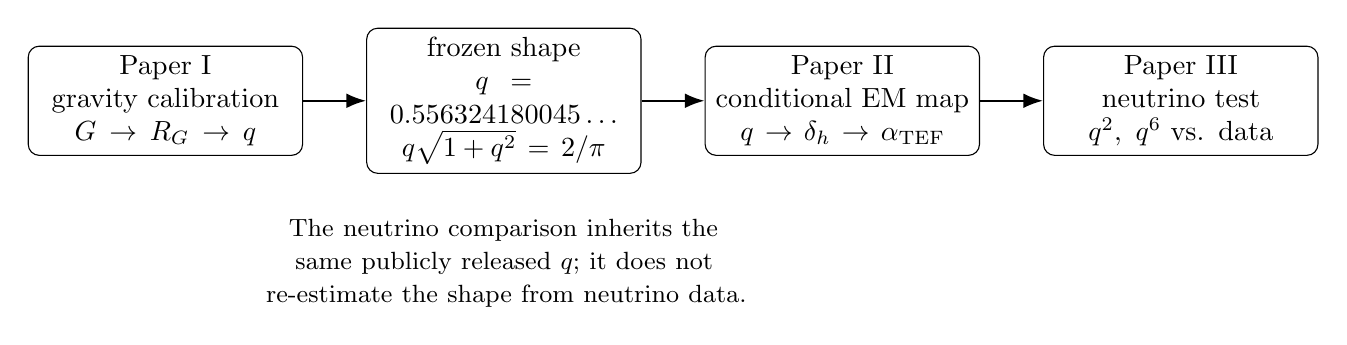
\begin{tikzpicture}[
 node distance=1.0cm and 0.8cm,
 box/.style={draw,rounded corners,align=center,minimum height=0.95cm,text width=3.25cm},
 arr/.style={-{Latex[length=2.5mm]},thick}
]
\node[box] (I) {Paper I\\gravity calibration\\$G\to R_G\to q$};
\node[box,right=of I] (shape) {frozen shape\\$q=0.556324180045\ldots$\\$q\sqrt{1+q^2}=2/\pi$};
\node[box,right=of shape] (II) {Paper II\\conditional EM map\\$q\to\delta_h\to\alpha_{\TEF}$};
\node[box,right=of II] (III) {Paper III\\neutrino test\\$q^2,\ q^6$ vs. data};
\draw[arr] (I)--(shape);
\draw[arr] (shape)--(II);
\draw[arr] (II)--(III);
\node[below=0.45cm of shape,align=center,text width=6.5cm] {\small
The neutrino comparison inherits the same publicly released $q$; it does not
re-estimate the shape from neutrino data.};
\end{tikzpicture}
\caption{Logical continuity of the three TEF papers.  Arrows denote inheritance
or an explicitly conditional continuation, not a completed derivation of the
corresponding Standard-Model sector.}
\label{fig:sequence}
\end{figure*}

\section{Neutrino observables in the current experimental convention}
\label{sec:standard}

For relativistic vacuum propagation, the standard oscillation phase contains
\begin{equation}
\Delta\phi_{ij}
\simeq
\frac{\Delta m^2_{ij}L}{2E},
\qquad
\Delta m^2_{ij}=m_i^2-m_j^2.
\label{eq:phase}
\end{equation}
The present paper does not require a microscopic interpretation of $m_i$ as a
primitive TEF object.  It uses the reported mass-squared differences as
operationally defined propagation invariants.

To avoid switching definitions between normal and inverted ordering, define
\begin{equation}
\boxed{
\rnu
\equiv
\frac{\Delta m^2_{21}}{|\Delta m^2_{3\ell}|},
}
\label{eq:rnu}
\end{equation}
with the NuFIT convention
\begin{equation}
\Delta m^2_{3\ell}
=
\begin{cases}
\Delta m^2_{31}, & \text{normal ordering (NO)},\\
\Delta m^2_{32}, & \text{inverted ordering (IO)}.
\end{cases}
\end{equation}
The first JUNO result fixes the numerator in
Eq.~\eqref{eq:rnu}.  For a conservative comparison of the denominator, we use
the NuFIT~6.1 global values quoted without the added atmospheric
$\chi^2$ tables~\cite{Esteban2026}:
\begin{align}
\Delta m^2_{31}\big|_{\rm NO}
&=
2.521^{+0.026}_{-0.018}
\times10^{-3}\ \mathrm{eV}^2,
\label{eq:no31}\\
\Delta m^2_{32}\big|_{\rm IO}
&=
-2.510^{+0.024}_{-0.023}
\times10^{-3}\ \mathrm{eV}^2.
\label{eq:io32}
\end{align}
This choice is useful because the NuFIT analysis in this variant uses the
published JUNO information for the solar parameters but does not use JUNO's
fast-oscillation information to determine $\Delta m^2_{3\ell}$.

The resulting central ratios are
\begin{align}
\rnu^{\rm NO}
&=0.0297501,
\label{eq:rno}\\
\rnu^{\rm IO}
&=0.0298805.
\label{eq:rio}
\end{align}
A conservative rectangular endpoint envelope of the quoted one-dimensional
marginal errors gives
\begin{align}
\rnu^{\rm NO}
&=0.029750^{+0.000693}_{-0.000775},\\
\rnu^{\rm IO}
&=0.029880^{+0.000771}_{-0.000745}.
\end{align}
For IO, taking the absolute value of the negative
$\Delta m^2_{32}$ reverses the direction of its quoted asymmetric errors.
The endpoint envelope is not a standard one-dimensional $68\%$ confidence
interval.  If the published marginals are instead treated provisionally as
independent near-Gaussian inputs, linear quadrature gives the orientation
estimates
\begin{align}
\rnu^{\rm NO}
&\simeq0.0297501^{+0.000521}_{-0.000566},\\
\rnu^{\rm IO}
&\simeq0.0298805^{+0.000557}_{-0.000551}.
\end{align}
Neither approximation replaces a joint likelihood or covariance analysis.

\section{Cross-sector numerical observations}
\label{sec:numerics}

\subsection{Observation I: the solar mixing number}

The first simple descendant of the frozen shape is
\begin{equation}
\boxed{
q^2=\qsql\ldots
}
\label{eq:q2}
\end{equation}
which may be placed beside JUNO's
Eq.~\eqref{eq:juno-theta}.  The central-value difference is
\begin{equation}
q^2-0.3092
=2.97\times10^{-4},
\end{equation}
about $0.096\%$ of the JUNO central value and approximately
$0.034$ of its quoted $1\sigma$ uncertainty.

The corresponding amplitude-level rewriting is
\begin{equation}
q\simeq\sin\theta_{12}.
\label{eq:qsin}
\end{equation}
Equation~\eqref{eq:qsin} is not derived from a neutrino Hamiltonian.  It is the
minimal reading of Eq.~\eqref{eq:q2} if $q$ is associated with an amplitude whose
experimentally reported quantity is squared.  A future theory would have to
produce the relevant interaction/propagation basis overlap rather than insert it
by definition.

\subsection{Observation II: the splitting hierarchy}

The sixth power of the same shape is
\begin{equation}
\boxed{
q^6=\qsix\ldots .
}
\label{eq:q6}
\end{equation}
Compared with Eqs.~\eqref{eq:rno}--\eqref{eq:rio}, the differences in central
values are approximately $0.35\%$ for NO and $0.78\%$ for IO.  Both are comfortably
inside current uncertainties; the present comparison therefore has no useful
mass-ordering discrimination.

If one uses the JUNO value of $\Delta m^2_{21}$ as a scale input, the
correspondence $\rnu\simeq q^6$ implies for NO
\begin{equation}
\Delta m^2_{31}
\simeq
\frac{\Delta m^2_{21}}{q^6}
=
2.52984\times10^{-3}\ \mathrm{eV}^2,
\label{eq:conditional31}
\end{equation}
close to Eq.~\eqref{eq:no31}.  Conversely, using the NuFIT NO denominator gives
\begin{equation}
\Delta m^2_{21}
\simeq
q^6\Delta m^2_{31}
=
7.474\times10^{-5}\ \mathrm{eV}^2,
\label{eq:conditional21}
\end{equation}
close to Eq.~\eqref{eq:juno-dm21}.  These are conditional restatements of one
ratio correspondence, not independent predictions.

\begin{table*}[t]
\centering
\caption{Cross-sector comparison from the frozen TEF shape.  Experimental
quantities are not used to reoptimize $q$.  The mappings $q^2$ and $q^6$ were
recognized after the neutrino sector was examined and therefore remain
phenomenological.}
\label{tab:numerics}
\begin{tabular}{@{}p{3.5cm}p{3.4cm}p{3.2cm}p{4.2cm}@{}}
\toprule
Quantity & TEF descendant & TEF value & Current comparison\\
\midrule
Solar mixing
& $q^2$
& $0.3094965933$
& JUNO: $\sin^2\theta_{12}=0.3092\pm0.0087$\\[0.45em]
NO splitting ratio
& $q^6$
& $0.0296461034$
& $\rnu^{\rm NO}=0.029750^{+0.000693}_{-0.000775}$\\[0.45em]
IO splitting ratio
& $q^6$
& $0.0296461034$
& $\rnu^{\rm IO}=0.029880^{+0.000771}_{-0.000745}$\\[0.45em]
Conditional NO large splitting
& $\Delta m^2_{21}/q^6$
& $2.52984\times10^{-3}\ \mathrm{eV}^2$
& NuFIT~6.1: $2.521^{+0.026}_{-0.018}\times10^{-3}\ \mathrm{eV}^2$\\
\bottomrule
\end{tabular}
\end{table*}

\subsection{The parameter-eliminated relation}

If the two observations share one origin, eliminating $q$ yields
\begin{equation}
\boxed{
\rnu
\simeq
\sin^6\theta_{12}.
}
\label{eq:master}
\end{equation}
Equivalently,
\begin{equation}
\sqrt{\rnu}
\simeq
\sin^3\theta_{12}.
\label{eq:masterroot}
\end{equation}
This is the cleanest phenomenological statement because it can be tested without
accepting TEF.  It is not a third independent numerical success: it follows
algebraically from the two frozen mappings after eliminating $q$ and is retained
for its value as a prospective parameter-eliminated test.  With the first JUNO central value,
\begin{equation}
(\sin^2\theta_{12})^3
=0.02956095.
\end{equation}
A linear propagation of JUNO's present $\theta_{12}$ uncertainty gives roughly
$0.00250$, much wider than the uncertainty on the splitting ratio.  Thus the
current agreement of Eq.~\eqref{eq:master} is suggestive but statistically weak;
the relation becomes more discriminating primarily as $\theta_{12}$ precision
improves.

\subsection{Discovery-order and search-space disclosure}

The sequence of inference matters:
\begin{enumerate}
\item $q$ was fixed in Paper~I and publicly released before the present neutrino
comparison;
\item Paper~II reused the same $q$ in an electromagnetic correspondence;
\item the neutrino sector was then selected on qualitative electroweak grounds;
\item the mappings $q^2$ and $q^6$ were recognized after examining neutrino
oscillation observables.
\end{enumerate}
Hence the value of $q$ is out-of-sector, but the mapping functions are not
preregistered predictions.  This paper does not assign a formal look-elsewhere
$p$-value because the historical search space was not defined prospectively.

It instead freezes the two relations at the present stage: no alternative
exponent, multiplicative correction, or new function of $q$ is introduced to
repair future disagreement.

\begin{table}[t]
\centering
\caption{Frozen mapping ledger from the present paper onward.  These choices define
the prospective comparison and are not to be retuned after future data updates.}
\label{tab:ledger}
\begin{tabular}{@{}p{2.65cm}p{4.35cm}@{}}
\toprule
Item & Frozen choice\\
\midrule
Upstream parameter & $q=0.556324180045\ldots$\\
Angle observable & $\sin^2\theta_{12}$\\
Angle map & $q^2$\\
Splitting observable & $\Delta m^2_{21}/|\Delta m^2_{3\ell}|$\\
Splitting map & $q^6$\\
Convention & NuFIT $3\ell$ convention\\
Ordering & NO and IO both reported\\
Future retuning & none\\
\bottomrule
\end{tabular}
\end{table}

\section{The geometric status of the frozen parameter}
\label{sec:geometry}

\subsection{A stronger intrinsic identity: \texorpdfstring{$q=\tau/\kappa$}{q=tau/kappa}}

For the circular helix in Eq.~\eqref{eq:helix}, the Frenet--Serret curvature and
torsion are
\begin{align}
\kappa
&=
\frac{R}{R^2+a^2},\\
\tau
&=
\frac{a}{R^2+a^2}.
\end{align}
Therefore
\begin{equation}
\boxed{
q
=
\frac{a}{R}
=
\frac{\tau}{\kappa}.
}
\label{eq:qtk}
\end{equation}
For the Euclidean circular-helix ansatz in $\mathbb R^3$, this identity is exact
differential geometry and does not depend on the neutrino comparison.  It
strengthens the interpretation of $q$: the frozen TEF number is not only a
pitch-to-radius ratio but also the dimensionless Frenet--Serret ratio of local
twisting to local bending.  No claim is made here that this Euclidean curve ratio
is already a Lorentzian spacetime invariant.

The symbol $\tau$ here is \emph{Frenet--Serret torsion of an embedded curve}.
It must not be confused with spacetime torsion in Riemann--Cartan or
Einstein--Cartan geometry, where torsion is a tensor associated with an affine
connection.  The two notions share terminology but are mathematically distinct.
This distinction is especially important because there is already a neutrino
literature on Einstein--Cartan torsion, discussed below.

\subsection{Why \texorpdfstring{$q^3$}{q3} is only a clue}

The identity
\begin{equation}
q^6=(q^3)^2
\end{equation}
invites a three-dimensional interpretation.  An isotropic map
$(x,y,z)\mapsto(qx,qy,qz)$ has Jacobian $q^3$.  However, a volume Jacobian and an
eigenvalue-gap amplitude are different mathematical objects.  No result in the
present TEF ansatz establishes
\begin{equation}
q^3
=
\sqrt{\frac{\Delta m^2_{21}}{|\Delta m^2_{3\ell}|}}.
\end{equation}
Accordingly, the decomposition $q^6=(q^3)^2$ is retained only as a suggestive
three-dimensional geometric clue.  In the absence of a derived spectral
connection, it is not treated as a theoretical explanation of the neutrino
splitting ratio.

\subsection{The spectral problem created by the observations}

The natural mathematical target is no longer another numerical formula.  It is a
single operator derived from the same three-dimensional geometry.
To avoid ambiguity about whether an eigenvalue is a mass, a frequency, or already
a squared invariant, it is useful to state the future target directly in terms of
a self-adjoint effective mass-squared or propagation-invariant operator,
\begin{equation}
\boxed{
\mathcal M_{\TEF}^{2}(q)\Psi_i
=
\mu_i(q)\Psi_i.
}
\label{eq:operator}
\end{equation}
A successful continuation would have to produce both the reduced solar-sector
mixing overlap and the appropriate splitting hierarchy.

In the standard three-flavor PMNS convention,
$|U_{e2}|=s_{12}c_{13}$ rather than $s_{12}$ itself.  The basis-invariant target
corresponding to the present $q^2$ observation is therefore
\begin{equation}
\boxed{
\frac{|U_{e2}|}
{\sqrt{|U_{e1}|^2+|U_{e2}|^2}}
=
\sin\theta_{12}
=
q,
}
\label{eq:vector-target}
\end{equation}
not the unnormalized statement $|U_{e2}|=q$.
Any two-state matrix written with entries
$\sqrt{1-q^2}$ and $q$ should consequently be interpreted only as a reduced
solar-sector rotation, not as the full PMNS matrix.

For normal ordering, the corresponding spectral target is
\begin{equation}
\boxed{
\frac{\mu_2-\mu_1}
{\mu_3-\mu_1}
=
q^6,
}
\label{eq:spectrum-target-no}
\end{equation}
whereas in the NuFIT inverted-ordering convention it becomes
\begin{equation}
\boxed{
\frac{\mu_2-\mu_1}
{|\mu_3-\mu_2|}
=
q^6.
}
\label{eq:spectrum-target-io}
\end{equation}
Equations~\eqref{eq:vector-target}--\eqref{eq:spectrum-target-io} are target
conditions, not deductions of the present paper.

Quantum mechanics on curved space curves provides a useful mathematical precedent
without supplying this neutrino operator.  Ortix derived an effective
Schr\"odinger--Pauli equation for a spin-orbit-coupled electron constrained to a
space curve and found curvature/torsion-dependent geometric terms, including an
explicit helical case~\cite{Ortix2015}.  More recently, Hou, Gao, and Guo showed
that retaining a degenerate transverse subspace in a curved quantum waveguide can
make Frenet-frame rotation generate a matrix-valued gauge connection controlled by
curve torsion~\cite{Hou2026}.  These systems are nonrelativistic constrained
waveguides, not neutrinos and not evidence for TEF.  Their relevance is narrower:
they demonstrate that Frenet--Serret data can enter a genuine quantum operator and
its spectrum.  The existence of torsion-dependent terms in such constrained
systems does not select the powers $q^2$ or $q^6$ and therefore does not by itself
explain either correspondence reported here.

\section{External research context}
\label{sec:literature}

The word ``geometric'' covers several very different research programs.  To locate
the present paper accurately, it is useful to separate at least five of them.

\subsection{Flavor symmetry and modular symmetry: the mainstream structural benchmark}

Most theoretical attempts to explain lepton mixing do not begin from a literal
three-dimensional curve.  They construct neutrino and charged-lepton mass matrices
from flavor symmetries, residual symmetries, seesaw structures, texture constraints,
or related mechanisms.  Modular flavor symmetry is a particularly active modern
example: the modular parameter and modular forms constrain Yukawa structures and
mixing matrices, often together with generalized CP symmetry~\cite{DingKing2024}.

This literature provides the appropriate benchmark for what a full TEF neutrino
theory would eventually need to achieve.  A mature model should not merely reproduce
one angle or one splitting ratio; it should specify the state space and operator or
mass structure from which the PMNS matrix, eigenvalue hierarchy, CP properties, and
matter-dependent propagation follow.  The present work does not meet that benchmark and
does not claim to.

\subsection{Geometric phenomenology of oscillation parameters}

A closer methodological comparator is Seikh's 2025 geometric hypothesis for
neutrino oscillation parameters~\cite{Seikh2025}.  That work proposes a Euclidean
triangle relation among the three mixing angles, treats it explicitly as an
empirical phenomenological organizing principle rather than a result of known
dynamics, and performs a consistency test against global-fit data.

The similarity is the willingness to state a compact, falsifiable geometric
relation before a microscopic mechanism is known.  The difference is the ancestry
of the organizing quantity.  Seikh constructs the geometric relation directly from
neutrino mixing angles, whereas the present $q$ was defined and numerically fixed in
a separate gravity-calibrated helix construction before the neutrino comparison.
This does not remove mapping-choice freedom, but it makes the present test genuinely
cross-sector.

\subsection{Topology and geometric phases in neutrino physics}

Topology has also entered neutrino theory in more microscopic ways.  Gu proposed a
model in which neutrinos are built from topological Majorana zero modes and used the
construction to address three generations and mixing~\cite{Gu2014}.  Separately,
geometric and topological phases have been studied within otherwise standard
neutrino oscillation kinematics, including two-flavor topological phases and
three-flavor gauge-invariant geometric phases~\cite{Mehta2009,Manosh2022}.

These works establish that neither ``topology and neutrinos'' nor ``geometry and
oscillation phase'' is a novelty claim available to TEF.  Their mechanisms are,
however, distinct from the present proposal.  The TEF observation concerns the
reuse of one dimensionless invariant of a prior microscopic helical-spacetime
ansatz and does not presently derive a Berry/Pancharatnam phase or a Majorana
zero-mode construction.

\subsection{Spacetime torsion and the terminological boundary}

There is also an active literature on neutrino oscillations in backgrounds with
spacetime torsion.  For example, Panda \emph{et al.} study modifications of the
oscillation Hamiltonian from torsional couplings in curved spacetime and assess
long-baseline sensitivities~\cite{Panda2024}.  Such models use torsion/contorsion of
the spacetime affine connection, commonly in an Einstein--Cartan-type setting.

Equation~\eqref{eq:qtk} concerns something different: $\tau$ is the Frenet--Serret
torsion of the TEF circular helix.  The present work therefore does not cite
Einstein--Cartan torsion as a derivation or precedent for $q=\tau/\kappa$; it cites
that literature to mark the distinction and to avoid a false equivalence.

\subsection{The 2026 Zenodo geometry--PMNS landscape}

Zenodo is a general-purpose repository rather than a peer-review filter.  Its
records are nevertheless useful for novelty checks because speculative geometry
and neutrino models often appear there before, or without, journal publication.
A targeted 2026 search finds several nearby examples.

McKoy's \emph{Neutrino Masses and PMNS Mixing Angles from SO(6) Boundary Geometry}
uses an $SO(6)$-based geometric construction to quote all three PMNS angles and an
absolute neutrino mass scale~\cite{McKoy2026}.  Jagadeesan's OOB series likewise
reports geometry-driven, nominally parameter-free PMNS values and explicitly
compares standing predictions with the first JUNO result~\cite{Jagadeesan2026}.
These deposits are useful comparators for the current speculative landscape, not
validation benchmarks.

The lesson for the present paper is methodological.  Geometry-based numerical
claims are easy to proliferate, especially when many algebraic expressions or
structural constants are available.  The TEF series therefore restricts its narrow
claim to the portability of one frozen upstream parameter and states explicitly
where a downstream mapping was recognized after the fact.

\subsection{Narrow novelty boundary}

A targeted, necessarily non-exhaustive search of arXiv and Zenodo through
29~August~2026 did not locate the exact phenomenological relation
\begin{equation}
\frac{\Delta m^2_{21}}{|\Delta m^2_{3\ell}|}
\simeq
\sin^6\theta_{12}
\end{equation}
or the specific use of the gravity-calibrated circular-helix invariant
\begin{equation}
q=\frac{a}{R}=\frac{\tau}{\kappa}
\end{equation}
as the common antecedent of the weak-angle, fine-structure, and neutrino
correspondences developed in the three TEF papers.  This is a limited novelty
statement about the present search, not a claim of priority for geometric or
topological approaches to neutrino mixing in general.

\section{Questions raised rather than solved}
\label{sec:questions}

The strongest version of the present result is a question, not an explanation.
The two numerical observations ask whether one microscopic geometric degree of
freedom can appear both in a state overlap and in a propagation spectrum.

\subsection{Can the helix generate the basis change?}

If Eq.~\eqref{eq:qsin} has physical content, a theory must explain why the
Frenet--Serret ratio $\tau/\kappa$ becomes the overlap between an
interaction-defined electron-neutrino state and a propagation eigenmode.  Writing
by hand the two-state matrix
\begin{equation}
\begin{pmatrix}
\sqrt{1-q^2} & q\\
-q & \sqrt{1-q^2}
\end{pmatrix}
\end{equation}
is algebraically consistent but does not answer the question.

\subsection{Can the same operator generate the gap ratio?}

The stronger constraints are Eqs.~\eqref{eq:spectrum-target-no} and \eqref{eq:spectrum-target-io}.  The same operator
must possess three relevant eigenmodes and must produce the measured hierarchy
without assigning the exponent six after seeing the data.  This requires a
boundary-value problem, an energy functional or relativistic wave operator, and a
clear identification of the measured oscillation phases.

\subsection{Why three active modes?}

The three-neutrino framework is an experimental input here, not a TEF result.  A
true topological completion should first classify the admissible modes and only
then identify three of them with $\nu_1,\nu_2,\nu_3$.  The same classification
would need to explain why the remaining PMNS parameters are not arbitrary.

\subsection{What would make the spacetime-mode hypothesis physical?}

One possible TEF interpretation, motivating but not required by the numerical
result, is that a neutrino is a propagating spinorial mode associated with emitted
spacetime structure.  To become physics rather than ontology, such a proposal must
recover at least the observed relativistic dispersion, weak chirality, $W/Z$
couplings, standard oscillation probabilities, matter effects, and the absence of
observable preferred-frame effects.  These derivations are beyond the scope of the present paper.

\section{Methodological boundaries and falsifiability}
\label{sec:falsify}

\subsection{Freeze the upstream quantity and the present mappings}

The value
\begin{equation}
q=0.556324180045\ldots
\end{equation}
is inherited from Paper~I and is not to be refitted to neutrino data.  From the
publication of the present analysis onward, the two reported mappings are also
treated as frozen empirical targets:
\begin{equation}
\sin^2\theta_{12}\stackrel{?}{=}q^2,
\qquad
\rnu\stackrel{?}{=}q^6.
\end{equation}
Future disagreement should not be repaired by changing the exponent, choosing a
new trigonometric function, or adding a fitted coefficient.

\subsection{Do not confuse cross-sector ancestry with a preregistered prediction}

Because $q$ was fixed upstream, the comparison is stronger than defining $q$ from
neutrino data.  But the functions $q^2$ and $q^6$ were recognized downstream.
Accordingly, the paper uses phrases such as ``cross-sector correspondence'' and
``coefficient-free conditional relation'' rather than claiming a parameter-free
first-principles prediction.

\subsection{Use ordering-safe and convention-explicit comparisons}

The ratio $\rnu$ in Eq.~\eqref{eq:rnu} is retained precisely to prevent a silent
switch among $\Delta m^2_{31}$, $\Delta m^2_{32}$, $\Delta m^2_{3\ell}$, and
$\Delta m^2_{ee}$.  Both NO and IO are shown.  Any future precision update should
use public likelihoods/covariances where available rather than treating all
reported errors as independent Gaussians.

\subsection{No search for the remaining PMNS parameters in this paper}

No new expression in $q$ is proposed for
$\theta_{13}$, $\theta_{23}$, or $\delta_{\rm CP}$.  Nor is $q$ used here to fit
the absolute neutrino mass scale.  The next meaningful advance is an operator or
topological classification that outputs additional observables without a new
post-hoc search.

\section{Discussion}

The three-paper TEF sequence now has a clearer logical shape.  Paper~I fixed a
microscopic helix using a gravity calibration and a cycle condition.  Paper~II
asked whether that frozen shape admits a conditional electromagnetic numerical
map, while explicitly separating exact geometry from postulates and conventions.
The present paper does not add a new primitive constant.  It asks whether the same
shape leaves a further trace in neutrino oscillation data.

The answer, as a numerical statement, is compact:
\begin{equation}
q^2=0.3094965933\ldots
\end{equation}
lies near the measured $\sin^2\theta_{12}$, while
\begin{equation}
q^6=0.0296461034\ldots
\end{equation}
lies near the measured small-to-large oscillation splitting ratio.  If both are
physical manifestations of the same structure, they imply
\begin{equation}
\rnu\simeq\sin^6\theta_{12}.
\end{equation}
At current precision this relation is compatible with the data but weakly tested,
primarily because the uncertainty propagated from $\theta_{12}$ remains broad.

An additional geometric observation is not another fitted formula but the exact
identity $q=\tau/\kappa$ for the Euclidean circular-helix ansatz.  It converts the inherited shape parameter into a ratio
of the two Frenet--Serret invariants of the circular helix.  Existing curved-curve
quantum mechanics shows that curvature and torsion can enter actual quantum
operators.  The research problem is therefore sharply stated: determine whether a
relativistic, spinorial, covariant TEF operator built from the same geometry can
produce both the required eigenvector overlap and the required eigenvalue-gap
ratio.  Until then, the two successful numbers remain phenomenology.

This placement also clarifies the relationship to the surrounding literature.
Mainstream flavor and modular-symmetry programs provide the standard of a true
mixing model; geometric phenomenology shows that compact empirical relations can
be scientifically testable before a mechanism is known; topology and geometric
phases are already established themes in neutrino research; and torsion-based
neutrino studies use a different mathematical torsion from the one entering the
TEF helix.  Zenodo contains additional 2026 geometry--PMNS proposals, which
reinforces the need for narrow novelty claims and explicit mapping-choice
accounting.

\section{Conclusion}

A gravity-calibrated helical-spacetime ansatz fixed the dimensionless shape
\begin{equation}
q=0.556324180045\ldots
\end{equation}
in the first TEF paper, before neutrino data were considered in this research
sequence.  A second TEF paper inherited the same shape in a conditional
fine-structure correspondence.  The present third paper carries that frozen
quantity into neutrino oscillation phenomenology and records
\begin{align}
q^2
&=0.3094965933\ldots
\simeq\sin^2\theta_{12},\\
q^6
&=0.0296461034\ldots
\simeq
\frac{\Delta m^2_{21}}{|\Delta m^2_{3\ell}|}.
\end{align}
The parameter-eliminated statement is
\begin{equation}
\boxed{
\frac{\Delta m^2_{21}}{|\Delta m^2_{3\ell}|}
\simeq
\sin^6\theta_{12}.
}
\end{equation}
It can be tested independently of TEF as neutrino precision improves.

The paper does not claim that neutrino mixing has been explained.  Its geometric
addition is the exact identity
\begin{equation}
q=\frac{a}{R}=\frac{\tau}{\kappa}
\end{equation}
for the inherited circular helix, which turns the frozen number into a
Frenet--Serret invariant ratio and motivates, but does not supply, a spectral
mechanism.  The unresolved problem is whether one operator derived from that same
three-dimensional structure can generate both the relevant state overlap and the
propagation-gap hierarchy.

The appropriate status of the result is therefore deliberately modest: a
cross-sector numerical correspondence produced by a previously released geometric
parameter, embedded in the contemporary neutrino literature and converted into a
specific dynamical question.  If future data reject either frozen relation, the
correspondence fails.  If a common spectral mechanism can be derived without
reoptimizing the mappings, the numerical observation would acquire a qualitatively
different theoretical status.

\section*{Acknowledgments}

The author thanks the experimental neutrino and precision-physics communities for
making high-quality reference data publicly available, and the mathematical-physics
community for developing geometric tools against which speculative microscopic
models can be formulated and tested.

\begin{thebibliography}{99}

\bibitem{WuI}
X.~Wu,
``A Helical Spacetime Ansatz Linking the Planck Scale and Electroweak Mixing,''
Version 5.1 (2026), Zenodo,
\href{https://doi.org/10.5281/zenodo.22101000}{doi:10.5281/zenodo.22101000}.

\bibitem{WuII}
X.~Wu,
``From a Gravity-Calibrated Helix to a Conditional Fine-Structure Correspondence,''
Version 4.7 (2026), Zenodo,
\href{https://doi.org/10.5281/zenodo.22117153}{doi:10.5281/zenodo.22117153}.

\bibitem{MNS1962}
Z.~Maki, M.~Nakagawa, and S.~Sakata,
``Remarks on the Unified Model of Elementary Particles,''
\emph{Prog. Theor. Phys.} \textbf{28}, 870--880 (1962).

\bibitem{SuperK1998}
Y.~Fukuda \emph{et al.} (Super-Kamiokande Collaboration),
``Evidence for Oscillation of Atmospheric Neutrinos,''
\emph{Phys. Rev. Lett.} \textbf{81}, 1562--1567 (1998),
arXiv:hep-ex/9807003,
\href{https://doi.org/10.1103/PhysRevLett.81.1562}
{doi:10.1103/PhysRevLett.81.1562}.

\bibitem{JUNO2026}
JUNO Collaboration,
``Measurement of reactor neutrino oscillation with the first JUNO data,''
\emph{Nature} \textbf{654}, 343--348 (2026),
\href{https://doi.org/10.1038/s41586-026-10538-z}
{doi:10.1038/s41586-026-10538-z}.

\bibitem{Esteban2026}
I.~Esteban, M.~C.~Gonzalez-Garcia, M.~Maltoni, I.~Martinez-Soler,
J.~P.~Pinheiro, and T.~Schwetz,
``Lessons from the first JUNO results,''
\emph{JHEP} \textbf{04}, 089 (2026),
arXiv:2601.09791,
\href{https://doi.org/10.1007/JHEP04(2026)089}
{doi:10.1007/JHEP04(2026)089}.

\bibitem{DingKing2024}
G.-J.~Ding and S.~F.~King,
``Neutrino mass and mixing with modular symmetry,''
\emph{Rep. Prog. Phys.} \textbf{87}, 084201 (2024),
arXiv:2311.09282,
\href{https://doi.org/10.1088/1361-6633/ad52a3}
{doi:10.1088/1361-6633/ad52a3}.

\bibitem{Seikh2025}
M.~F.~H.~Seikh,
``A geometrical approach to neutrino oscillation parameters,''
\emph{AIP Advances} \textbf{15}, 105204 (2025),
arXiv:2510.06526,
\href{https://doi.org/10.1063/5.0292233}{doi:10.1063/5.0292233}.

\bibitem{Gu2014}
Z.-C.~Gu,
``Neutrino as topological Majorana zero modes: the origin of three generations of
neutrinos and their mass mixing,''
arXiv:1403.1869 (2014).

\bibitem{Mehta2009}
P.~Mehta,
``Topological phase in two flavor neutrino oscillations,''
arXiv:0901.0790 (2009).

\bibitem{Manosh2022}
T.~M.~Manosh, N.~Shaji, R.~B.~Thayyullathil, and T.~K.~Mathew,
``Geometric phases in neutrino mixing,''
arXiv:2212.08245 (2022).

\bibitem{Panda2024}
P.~Panda, D.~K.~Singha, M.~Ghosh, and R.~Mohanta,
``Effect of torsion in long-baseline neutrino oscillation experiments,''
arXiv:2403.09105 (2024).

\bibitem{Ortix2015}
C.~Ortix,
``Quantum mechanics of a spin-orbit coupled electron constrained to a space curve,''
\emph{Phys. Rev. B} \textbf{91}, 245412 (2015),
arXiv:1504.00840,
\href{https://doi.org/10.1103/PhysRevB.91.245412}
{doi:10.1103/PhysRevB.91.245412}.

\bibitem{Hou2026}
X.-Y.~Hou, X.~Gao, and H.~Guo,
``Torsion-induced gauge structure in curved quantum waveguides,''
arXiv:2606.03725 (2026).

\bibitem{McKoy2026}
C.~McKoy,
``Neutrino Masses and PMNS Mixing Angles from SO(6) Boundary Geometry,''
Zenodo preprint, Version v1 (2026),
\href{https://doi.org/10.5281/zenodo.19411918}
{doi:10.5281/zenodo.19411918}.

\bibitem{Jagadeesan2026}
B.~D.~Jagadeesan,
``One-Octonion Brane-Bulk Framework --- Paper CCCXIII: PMNS Confirmation Note ---
JUNO theta-12 and T2K+NOvA theta-23 Land on the Parameter-Free OOB Values,''
Zenodo, Version 1.0 (2026),
\href{https://doi.org/10.5281/zenodo.20753387}
{doi:10.5281/zenodo.20753387}.

\end{thebibliography}

\end{document}
